\documentclass[11pt]{article}
\usepackage[top=1in]{geometry}
\usepackage{ebgaramond}
\usepackage{markdown}
\usepackage{enumitem}
\setlist{itemsep=1pt}

% use tikz
\usepackage{tikz}
\usetikzlibrary{positioning, fit, arrows.meta, shapes, calc, backgrounds}

\tikzset{
  node/.style={rectangle, draw, thick, rounded corners=3pt,
    minimum width=1.0cm, minimum height=0.9cm,
    font=\sffamily, align=center},
}

\begin{document}
\title{Generality}
\author{Ankush Jain}
\maketitle

\begin{figure}[h]
  \centering
  
\begin{tikzpicture}
    \node (A) [node] {A};
    \node (B) [node, right=of A.east] {B};
    \node (C) [node, right=of B.east] {C};
    \node (D) [node, right=of C.east] {D};
  \end{tikzpicture}
\end{figure}

% Observability is \begin{markdown} 1. a 2. b \end{markdown}

\section{What is Steerable Observability?}

An umbrella term for different usecases:

\begin{enumerate}
    \item \emph{Characterizing}, to formulate a model of system behavior.
    \item \emph{Monitoring}, to flag deviations from model.
    \item For observed deviations,
    \begin{itemize}
        \item If \emph{known}, facilitate online fixes if viable. Example: bad node found, facilitate live migration if supported. Out of scope if fix is manual (terminate, prune, restart).
        \item If \emph{unknown}, facilitate offline investigation via snapshots of system state (the \emph{crime scene}).
    \end{itemize}
\end{enumerate}

\subsection{Types of Anomalies}

\begin{enumerate}
    \item \emph{Known, Monitorable} e.g. thermal throttling
    \item \emph{Known, Unmonitorable} e.g. cosmic rays
    \item \emph{Unknown}: everything else
\end{enumerate}

\begin{figure}[h]
  \centering
  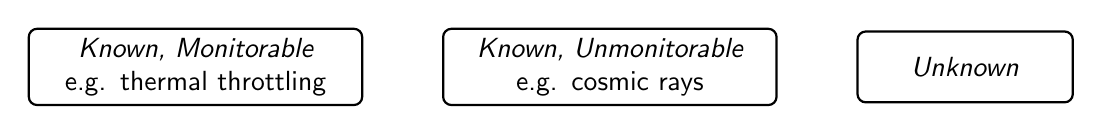
\begin{tikzpicture}
    \node (A) [node, text width=4.0cm] {\emph{Known, Monitorable} e.g. thermal throttling};
    \node (B) [node, text width=4.0cm, right=of A.east] {\emph{Known, Unmonitorable} e.g. cosmic rays};
    \node (C) [node, text width=2.5cm, right=of B.east] {\emph{Unknown}};

  \end{tikzpicture}
\end{figure}

\subsection{Enabling Investigation}

Investigation is fundamentally about navigating causal graphs, from symptom to cause.
This creates a challenge: \emph{what happened} can only be captured apriori.
Luckily, there is a difference between the minimal and maximal definitions of \emph{capture}:

\begin{itemize}
  \item Capturing events to local memory
  \item Serializing and transporting it over a message bus, and persisting it to a database or shared storage
\end{itemize}

\end{document}